\section{RenamableLogootSplit}

\subsection{Réplication de données dans systèmes pair-à-pair}

\begin{frame}{MUTE, un exemple de Local-First Software (LFS) \cite{localfirstsoftware2019}}
    \vspace{-0.5cm}
    \begin{figure}
        \resizebox{\textwidth}{!}{
            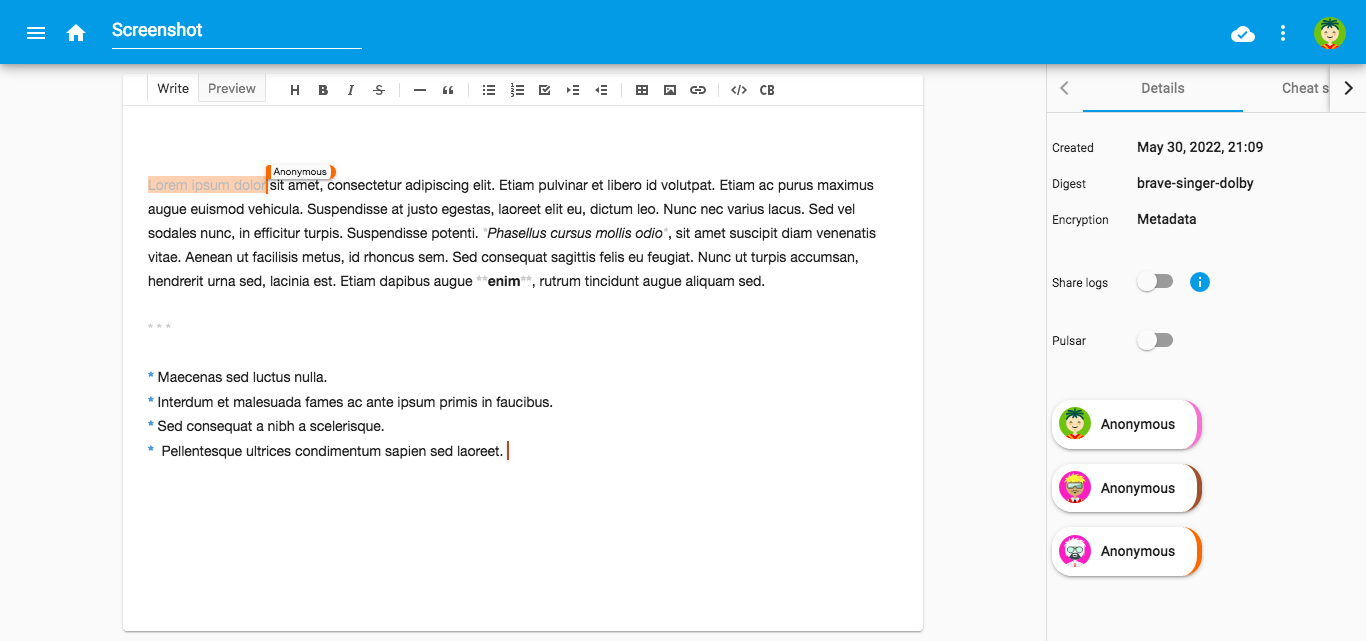
\includegraphics{img/screenshot-mute-editor.png}
        }
    \end{figure}
    \vspace{-0.5cm}
    \begin{itemize}
        \item Application pair-à-pair
        \item Permet de rédiger collaborativement des documents texte
        \item Garantit la confidentialité \& souveraineté des données
    \end{itemize}
\end{frame}

\begin{frame}[fragile]{Réplication dans applications collaboratives pair-à-pair}
    \begin{figure}
        \resizebox{0.7 \textwidth}{!}{
            \begin{tikzpicture}
                \newcommand{\doc}{
                    \tikz{
                        \fill[scale=.15,fill=white,draw=gray,thick,solid] (0,0) -- (7,0) -- (7,8) -- (5,10) -- (0,10) -- cycle;
                    }
                }
                \newcommand{\updsquare}{
                    \tikz{
                        \fill[\colorblockone, scale=.12] (0,0) rectangle (3,3);
                    }
                }
                \newcommand{\updcircle}{
                    \tikz{
                        \fill[\colorblocktwo, scale=.07] (3,3) circle (3);
                    }
                }
                \newcommand{\updtriangle}{
                    \tikz{
                        \fill[\colorblockfive, scale=.07] (0,0) -- (6,0) -- (3,6) -- cycle;
                    }
                }
                \path
                    node[label=90:{A}] (a) {
                        \includegraphics[scale=0.4, page=5, trim=0cm 24cm 32cm 0cm, clip]{img/mute-figures.pdf}
                    }
                    +(-70:3) node[label=-90:{B}] (b) {
                        \includegraphics[scale=0.4, page=5, trim=0cm 24cm 32cm 0cm, clip]{img/mute-figures.pdf}
                    }
                    +(200:4) node[label=-90:{C}] (c) {
                        \includegraphics[scale=0.4, page=5, trim=0cm 24cm 32cm 0cm, clip]{img/mute-figures.pdf}
                    };

                \path
                    (a) node[label={[xshift=2em]0:{\doc}}] {}
                    (b) node[label={[xshift=2em]0:{\doc}}] {}
                    (c) node[label={[xshift=-2em]180:{\doc}}] {};

                \onslide<4->{
                    \path
                        (a) node[label={[xshift=3.8em]90:{\updsquare}}] {}
                        (b) node[label={[xshift=3.7em]0:{\updtriangle}}] {}
                        (c) node[label={[xshift=-4.8em]-90:{\updcircle}}] {};
                }

                \onslide<5->{
                    \draw[dotted] (a) -- (b);
                }

                \only<6>{
                    \path
                        (a) -- node[midway]{
\includegraphics[scale=0.4]{img/sync.pdf}} (b);
                }

                \onslide<7->{
                    \path
                        (a) node[label={[xshift=3.7em]0:{\updtriangle}}] {}
                        (b) node[label={[xshift=3.8em]90:{\updsquare}}] {};
                }

                \onslide<8->{
                    \draw[dotted] (a) -- (c);
                    \draw[dotted] (b) -- (c);
                }

                \only<8> {
                    \path
                        (a) -- node[midway]{
\includegraphics[scale=0.4]{img/sync.pdf}} (c)
                        (b) -- node[midway]{
\includegraphics[scale=0.4]{img/sync.pdf}} (c);
                }

                \onslide<9->{
                    \path
                        (a) node[label={[xshift=3.8em]-90:{\updcircle}}] {}
                        (b) node[label={[xshift=3.8em]-90:{\updcircle}}] {}
                        (c) node[label={[xshift=-4.8em]90:{\updsquare}}] {}
                        (c) node[label={[xshift=-4.8em]0:{\updtriangle}}] {};
                }
            \end{tikzpicture}
        }
    \end{figure}
    \vspace{-1em}
    \begin{columns}
        \hspace{0em}
        \begin{column}{0.6\textwidth}
            \begin{itemize}
                \item<2-> Noeuds peuvent être \alert{déconnectés}
                \item<3-> Doivent pouvoir \alert{travailler sans coordination synchrone} préalable (par ex. consensus)
            \end{itemize}
        \end{column}
        \begin{column}{0.6\textwidth}
            \begin{itemize}
                \item<9-> Doit garantir \alert{cohérence à terme} \cite{10.1145/224057.224070}\dots
                \item<9-> \dots malgré ordres différents d'intégration des modifications
            \end{itemize}
        \end{column}
    \end{columns}
    \onslide<10>{
        \vspace{1em}
        \begin{center}
            \alert{Nécessite des \emph{mécanismes de résolution de conflits}}
        \end{center}
    }
\end{frame}

% \begin{frame}{Évaluation de MUTE}
%     \metroset{block=transparent}
%     \begin{block}{Taille du texte comparée à taille de la séquence répliquée}
%         \begin{columns}
%             \begin{column}{0.6\textwidth}
%                 \begin{figure}
%                     \resizebox{\columnwidth}{!}{
%                         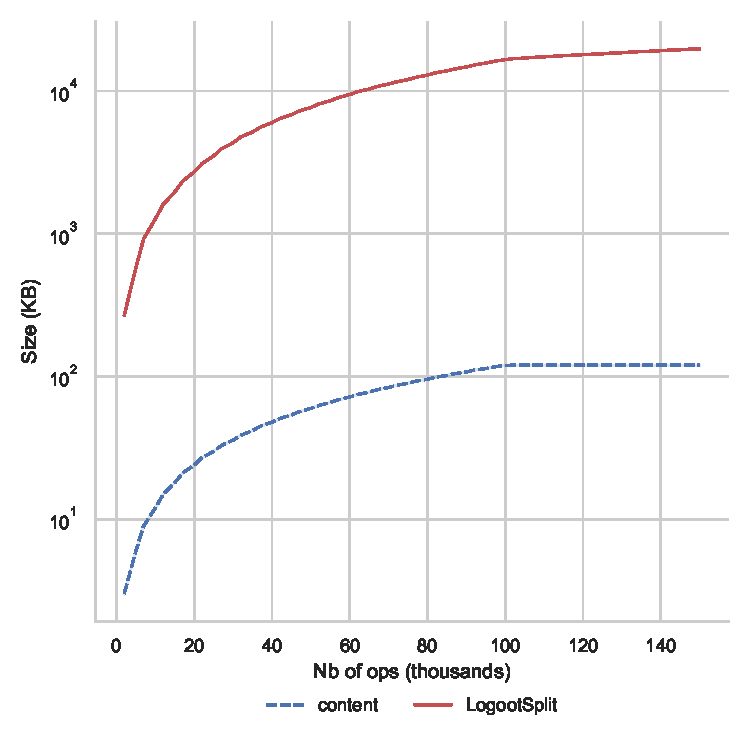
\includegraphics{img/ls-vs-content-snapshot-sizes-7k5.pdf}
%                     }
%                 \end{figure}
%             \end{column}
%             \begin{column}{0.4\textwidth}
%                 \pause
%                 \begin{block}{Constat}
%                     \begin{itemize}
%                         \item 1\% contenu\dots
%                         \item \dots 99\% métadonnées
%                     \end{itemize}
%                 \end{block}
%                 \pause
%                 \begin{center}
%                     \alert{Et ça augmente !}
%                 \end{center}
%                 \pause
%                 \begin{block}{Impact}
%                     \begin{itemize}
%                         \item Surcoût \alert{mémoire}\dots
%                         \item \dots mais aussi surcoût en \alert{calculs} et en \alert{bande-passante}
%                     \end{itemize}
%                 \end{block}
%             \end{column}
%         \end{columns}
%     \end{block}
% \end{frame}

% \begin{frame}[standout]
%     Comment peut-on \alert{réduire le surcoût} des mécanismes de résolution de conflits dans les applications pair-à-pair ?
% \end{frame}

\subsection{Conflict-free Replicated Data Types (CRDTs) pour le type Séquence}

\begin{frame}{Conflict-free Replicated Data Types (CRDTs)  \cite{shapiro_2011_crdt}}
    \begin{itemize}
        \item Nouvelles spécifications des types de données, \eg \emph{Ensemble} ou \emph{Séquence}
        \item Incorpore nativement mécanisme de résolution de conflits
    \end{itemize}
    \pause
    \begin{block}{Propriétés des CRDTs}
        \begin{itemize}
            \item Permettent modifications \alert{sans coordination}
            \item Garantissent la \alert{cohérence forte à terme}
        \end{itemize}
    \end{block}
    \pause
    \begin{block}{Cohérence forte à terme}
        Ensemble des noeuds ayant intégrés le même ensemble de modifications obtient des états équivalents, \alert{sans nécessiter d'actions ou messages supplémentaires}
    \end{block}
\end{frame}

\begin{frame}[fragile]{CRDTs pour le type Séquence}
    \metroset{block=transparent}
    \begin{columns}
        \begin{column}{0.6\textwidth}
            \begin{block}{\quad Type Séquence usuel}
                \begin{figure}[!ht]
                    \centering
                    \resizebox{\columnwidth}{!}{
                        \begin{tikzpicture}
                            \newcommand\initialstate[2]{
                                \path
                                    #1
                                    ++#2
                                    node[letter, label=below:{$0$}] {B}
                                    ++(0:\widthletter) node[letter, label=below:{$1$}] {N}
                                    ++(0:\widthletter) node[letter, label=below:{$2$}] {J}
                                    ++(0:\widthletter) node[letter, label=below:{$3$}] {O};
                            }
                            \newcommand\totoa[2]{
                                \path
                                    #1
                                    ++#2
                                    node[letter, label=below:{$0$}] {}
                                    ++(0:\widthletter) node[letter, label=below:{$1$}] {}
                                    ++(0:\widthletter) node[letter, label=below:{$2$}] {}
                                    ++(0:\widthletter) node[letter, label=below:{$3$}] {}
                                    ++(0:\widthletter) node[letter, label=below:{$4$}] {};
                            }
                            \newcommand\totob[2]{
                                \path
                                    #1
                                    ++#2
                                    node[letter, label=below:{$0$}] {B}
                                    ++(0:\widthletter) node[letter, label=below:{$1$}] {}
                                    ++(0:\widthletter) node[letter, label=below:{$2$}] {N}
                                    ++(0:\widthletter) node[letter, label=below:{$3$}] {J}
                                    ++(0:\widthletter) node[letter, label=below:{$4$}] {O};
                            }
                            \newcommand\totoc[2]{
                                \path
                                    #1
                                    ++#2
                                    node[letter, label=below:{$0$}] {B}
                                    ++(0:\widthletter) node[letter, label=below:{$1$}] {A}
                                    ++(0:\widthletter) node[letter, label=below:{$2$}] {N}
                                    ++(0:\widthletter) node[letter, label=below:{$3$}] {J}
                                    ++(0:\widthletter) node[letter, label=below:{$4$}] {O};
                            }

                            \newcommand\offseta{ (90:1) }

                            \path
                                node {\textbf{A}}
                                ++(0:0.5) node (a) {}
                                +(0:10) node (a-end) {}
                                +(0:1) node[point] (a-initial) {}
                                +(0:6) node (a-ins-a) {}
                                +(0:9) node (a-final) {};

                            \initialstate{(a-initial)}{\offseta};
                            \draw[dotted] (a) -- (a-initial) (a-final) -- (a-end);
                            \only<1>{
                                \draw[->, thick] (a-initial) -- (a-final);
                            }
                            \onslide<2->{
                                \path (a-ins-a) node[point, label=-170:{$\trm{ins}(1, A)$}] {};
                                \draw[->, thick] (a-initial) -- (a-ins-a) -- (a-final);
                            }
                            \only<3>{\totoa{(a-ins-a)}{\offseta}}
                            \only<4>{\totob{(a-ins-a)}{\offseta}}
                            \onslide<5->{\totoc{(a-ins-a)}{\offseta}}
                        \end{tikzpicture}
                    }
                \end{figure}
            \end{block}
        \end{column}
        \begin{column}{0.6\textwidth}
            \onslide<7->{
                \begin{block}{CRDTs pour Séquence}
                    \begin{figure}[!ht]
                        \centering
                        \resizebox{\columnwidth}{!}{
                            \begin{tikzpicture}
                                \newcommand\initialstate[2]{
                                    \path
                                        #1
                                        ++#2
                                        node[letter, label=below:{$\trm{id}_0$}] {B}
                                        ++(0:\widthletter) node[letter, label=below:{$\trm{id}_1$}] {N}
                                        ++(0:\widthletter) node[letter, label=below:{$\trm{id}_2$}] {J}
                                        ++(0:\widthletter) node[letter, label=below:{$\trm{id}_3$}] {O};
                                }
                                \newcommand\totoa[2]{
                                    \path
                                        #1
                                        ++#2
                                        node[letter, label=below:{}] {}
                                        ++(0:\widthletter) node[letter, label=below:{}] {}
                                        ++(0:\widthletter) node[letter, label=below:{}] {}
                                        ++(0:\widthletter) node[letter, label=below:{}] {}
                                        ++(0:\widthletter) node[letter, label=below:{}] {};
                                }
                                \newcommand\totob[2]{
                                    \path
                                        #1
                                        ++#2
                                        node[letter, label=below:{$\trm{id}_0$}] {B}
                                        ++(0:\widthletter) node[letter, label=below:{$?$}] {}
                                        ++(0:\widthletter) node[letter, label=below:{$\trm{id}_1$}] {N}
                                        ++(0:\widthletter) node[letter, label=below:{$\trm{id}_2$}] {J}
                                        ++(0:\widthletter) node[letter, label=below:{$\trm{id}_3$}] {O};
                                }
                                \newcommand\totoc[2]{
                                    \path
                                        #1
                                        ++#2
                                        node[letter, label=below:{$\trm{id}_0$}] {B}
                                        ++(0:\widthletter) node[letter, label=below:{$\trm{id}_{0.5}$}] {A}
                                        ++(0:\widthletter) node[letter, label=below:{$\trm{id}_1$}] {N}
                                        ++(0:\widthletter) node[letter, label=below:{$\trm{id}_2$}] {J}
                                        ++(0:\widthletter) node[letter, label=below:{$\trm{id}_3$}] {O};
                                }

                                \newcommand\offseta{ (90:1) }

                                \path
                                    node {\textbf{A}}
                                    ++(0:0.5) node (a) {}
                                    +(0:10) node (a-end) {}
                                    +(0:1) node[point] (a-initial) {}
                                    +(0:6) node (a-ins-a) {}
                                    +(0:9) node (a-final) {};

                                \initialstate{(a-initial)}{\offseta};
                                \draw[dotted] (a) -- (a-initial) (a-final) -- (a-end);
                                \only<7,8>{
                                    \draw[->, thick] (a-initial) -- (a-final);
                                }
                                \onslide<9->{
                                    \path (a-ins-a) node[point, label=-170:{$\trm{ins}(B \prec A \prec N)$}] {};
                                    \draw[->, thick] (a-initial) -- (a-ins-a) -- (a-final);
                                }
                                \only<9>{\totoa{(a-ins-a)}{\offseta}}
                                \only<10>{\totob{(a-ins-a)}{\offseta}}
                                \onslide<11->{\totoc{(a-ins-a)}{\offseta}}
                            \end{tikzpicture}
                        }
                    \end{figure}
                \end{block}
            }
        \end{column}
    \end{columns}
    \begin{itemize}
        \item<6-> Changements d'indices sont \alert{source de conflits}
        \item<7-> CRDTs assignent des \alert{identifiants de position} \cite{2009-treedoc-preguica} à chaque élément
        \item<7->
            Identifiants permettent d'\alert{ordonner les élements}
            \onslide<8->{
                \begin{equation*}
                    \trm{id}_0 \lid \trm{id}_1 \lid \trm{id}_2 \lid \trm{id}_3
                \end{equation*}
            }
        \vspace{-1.5em}
        \item<10->
            Identifiants appartiennent à un \alert{espace dense}
            \onslide<11->{
                \begin{equation*}
                    \trm{id}_0 \lid \trm{id}_{0.5} \lid \trm{id}_1
                \end{equation*}
            }
    \end{itemize}
    \vspace{-1em}
    \onslide<12->{
        \begin{center}
            \alert{Utilise LogootSplit \cite{2013-logootsplit} comme base}
        \end{center}
    }
\end{frame}

\begin{frame}{Identifiant LogootSplit}
    \metroset{block=transparent}
    \begin{block}{Identifiant}
        \begin{itemize}
            \item Composé d'\alert{un ou plusieurs tuples} de la forme
        \end{itemize}
        \vspace{3em}
        \begin{equation*}
            \tikzmarknode{pos}{pos}^{
                \tikzmarknode{nodeId}{nodeId}~\tikzmarknode{nodeSeq}{nodeSeq}
            }_{\tikzmarknode{offset}{offset}}
        \end{equation*}
        \begin{tikzpicture}[overlay,remember picture,>=stealth,nodes={align=left,inner ysep=1pt},<-]
            % For "pos"
            \path<2-> (pos.north) ++ (0,2em) node[anchor=south east,color=ucl1mdred] (legend-pos){\textbf{position (a-z)}};
            \draw<2-> [color=ucl1mdred](pos.north) |- ([xshift=-0.3ex,color=ucl1mdred] legend-pos.south west);
            % For "nodeId"
            \path<3-> (nodeId.north) ++ (0,2em) node[anchor=south west,color=ucl1mdblue] (legend-nodeid){\textbf{identifiant (A-Z) de l'auteur}};
            \draw<3-> [color=ucl1mdblue](nodeId.north) |- ([xshift=0.3ex,color=ucl1mdblue] legend-nodeid.south east);
            % For "nodeSeq"
            \path<4-> (nodeSeq.south) ++ (0,-2em) node[anchor=north west,color=ucl2dkpurple] (legend-nodeseq){\textbf{numéro de séquence (1-9)}};
            \draw<4-> [color=ucl2dkpurple](nodeSeq.south) |- ([xshift=0.3ex,color=ucl2dkpurple] legend-nodeseq.south east);
        \end{tikzpicture}
    \end{block}
    \onslide<5->{
        \begin{block}{Relation d'ordre $\lid$}
            \begin{itemize}
                \item Se base sur l'\alert{ordre lexicographique sur les éléments des tuples}
            \end{itemize}
        \end{block}
    }
    \onslide<6->{
        \begin{block}{Exemples}
            \begin{equation*}
                \id{
                    \only<8>{\mathbf{d}}
                    \only<6,7,9,10,11,12>{d}
                }{F5}{0}
                \onslide<7->{
                    \lid \id{
                        \only<7,9,10,11,12>{m}
                        \only<8>{\mathbf{m}}
                    }{C1}{0}
                }
                \onslide<9->{
                    \lid \id{m}{C1}{0}\id{
                        \only<9,11,12>{f}
                        \only<10>{\mathbf{f}}
                    }{
                        \only<9,11,12>{E1}
                        \only<10>{\mathbf{E1}}
                    }{
                        \only<9,11,12>{0}
                        \only<10>{\mathbf{0}}
                    }
                }
            \end{equation*}
            \onslide<11->{
                \begin{equation*}
                    \id{i}{B1}{0} \lid \only<11>{\quad?\quad} \only<12>{\id{i}{B1}{0}\alert{\id{f}{A1}{0}}} \lid \id{i}{B1}{1}
                \end{equation*}
            }
        \end{block}
    }
\end{frame}

\begin{frame}[fragile]{Bloc LogootSplit}
    \begin{itemize}
        \item Coûteux de stocker les identifiants de chaque élément
    \end{itemize}
    \begin{figure}[!ht]
        \begin{tikzpicture}
            \path
                node[letter, label=below:{$\id{m}{C1}{0}$}] {B}
                ++(0:\widthletter) node[letter, label=below:{$\id{m}{C1}{1}$}] {A}
                ++(0:\widthletter) node[letter, label=below:{$\id{m}{C1}{2}$}] {N}
                ++(0:\widthletter) node[letter, label=below:{$\id{m}{C1}{3}$}] {J}
                ++(0:\widthletter) node[letter, label=below:{$\id{m}{C1}{4}$}] {O};
        \end{tikzpicture}
    \end{figure}
    \pause
    \vspace{-1em}
    \begin{itemize}
        \item Aggrège en un \alert{bloc} éléments ayant \alert{identifiants contigus}
    \end{itemize}
    \begin{block}{Identifiants contigus}
        Deux identifiants sont contigus si et seulement si :
        \begin{enumerate}
            \item les deux identifiants sont identiques à l'exception de leur dernier offset
            \item ces deux derniers offsets sont consécutifs
        \end{enumerate}
    \end{block}
    \pause
    \begin{itemize}
        \item Note l'intervalle d'identifiants d'un bloc : $\id{pos}{nodeId~nodeSeq}{begin..end}$
    \end{itemize}
    \begin{figure}[!ht]
        \begin{tikzpicture}
            \path
                node[block, label=below:{$\id{m}{C1}{0..4}$}] {BANJO};
        \end{tikzpicture}
    \end{figure}
\end{frame}

\begin{frame}[fragile]{Exemple insertions concurrentes}
    \begin{columns}
        \hspace{0em}
        \begin{column}{1.1\textwidth}
            \begin{figure}[!ht]
                \centering
                \resizebox{\columnwidth}{!}{
                  \begin{tikzpicture}
                    \newcommand\nodehl[1]{
                        node[block, label=#1:{$\id{i}{B1}{0..1}$}] {HL}
                    }
                    \newcommand\nodehlo[1]{
                        node[block, label=#1:{$\id{i}{B1}{0..2}$}] {HLO}
                    }
                    \newcommand\nodeh[1]{
                        node[letter, label=#1:{$\id{i}{B1}{0}$}] {H}
                    }
                    \newcommand\nodee[1]{
                        node[letter, fill=\colorblockone, label=#1:{$\coloridone\id{i}{B1}{0}\id{f}{A1}{0}$}] {E}
                    }
                    \newcommand\nodel[1]{
                        node[letter, label=#1:{$\id{i}{B1}{1}$}] {L}
                    }
                    \newcommand\nodelo[1]{
                        node[block, label=#1:{$\id{i}{B1}{1..2}$}] {LO}
                    }

                    \newcommand\initialstate[3]{
                      \path
                        #1
                        ++#2
                        ++(0:0.5)
                        ++(#3:0.5) \nodehl{#3};
                    }

                    \newcommand\inso[3]{
                      \path
                        #1
                        ++#2
                        ++(0:0.5)
                        ++(#3:0.5) \nodehlo{#3};
                    }

                    \newcommand\inse[3]{
                      \path
                        #1
                        ++#2
                        ++(0:0.5)
                        ++(#3:0.5) \nodeh{#3}
                        ++(0:\widthletter) \nodee{#3}
                        ++(0:\widthletter) \nodel{#3};
                    }

                    \newcommand\finalstate[3]{
                      \path
                        #1
                        ++#2
                        ++(0:0.5)
                        ++(#3:0.5) \nodeh{#3}
                        ++(0:\widthletter) \nodee{#3}
                        ++(0:\widthletter) \nodelo{#3};
                    }

                    \newcommand\offseta{ (90:0.7) }
                    \newcommand\offsetb{ (270:0.7) }

                    \path
                        node {\textbf{A}}
                        ++(0:0.5) node (a) {}
                        +(0:16) node (a-end) {}
                        +(0:1) node[point] (a-initial) {}
                        +(0:5) node (a-ins-e) {}
                        +(0:10) node (a-recv-ins-o) {}
                        +(0:15) node (a-final) {};

                    \initialstate{(a-initial)}{\offseta}{90};
                    \draw[dotted] (a) -- (a-initial) (a-final) -- (a-end);

                    \path
                        ++(270:3) node {\textbf{B}}
                        ++(0:0.5) node (b) {}
                        +(0:16) node (b-end) {}
                        +(0:1) node[point] (b-initial) {}
                        +(0:5) node (b-ins-o) {}
                        +(0:10) node (b-recv-ins-e) {}
                        +(0:15) node (b-final) {};

                    \initialstate{(b-initial)}{\offsetb}{-90};
                    \draw[dotted] (b) -- (b-initial) (b-final) -- (b-end);

                    \only<1> {
                        \draw[->, thick] (a-initial) -- (a-final);
                    }
                    \only<1,2> {
                        \draw[->, thick] (b-initial) -- (b-final);
                    }
                    \only<2,3,4,5> {
                        \draw[->, thick] (a-initial) --  (a-ins-e) -- (a-final);
                    }
                    \onslide<2-> {
                        \path (a-ins-e) node[point, label=-170:{$\trm{ins}(H \prec E \prec L)$}] {};
                        \inse{(a-ins-e)}{\offseta}{90};
                    }
                    \only<3,4> {
                        \draw[->, thick] (b-initial) --  (b-ins-o) -- (b-final);
                    }
                    \onslide<3-> {
                        \path (b-ins-o) node[point, label=170:{$\trm{ins}(L \prec O)$}] {};
                        \inso{(b-ins-o)}{\offsetb}{-90};
                    }
                    \onslide<4-> {
                        \path (a-ins-e) node[label={[xshift=25pt]-10:{$\trm{ins}({\coloridthree\id{i}{B1}{0}\id{f}{A1}{0}},E)$}}] {};
                        \draw[->, dashed, shorten >= 1] (a-ins-e) -- (b-recv-ins-e);
                    }
                    \onslide<5-> {
                        \path (b-recv-ins-e) node[point] {};
                        \finalstate{(b-recv-ins-e)}{\offsetb}{-90};
                        \draw[->, thick] (b-initial) --  (b-ins-o) -- (b-recv-ins-e) -- (b-final);
                    }
                    \onslide<6-> {
                        \path (b-ins-o) node[label={[xshift=25pt]10:{$\trm{ins}(\id{i}{B1}{2},O)$}}] {};
                        \path (a-recv-ins-o) node[point] {};
                        \draw[->, dashed, shorten >= 1] (b-ins-o) -- (a-recv-ins-o);
                        \finalstate{(a-recv-ins-o)}{\offseta}{90};
                        \draw[->, thick] (a-initial) --  (a-ins-e) -- (a-recv-ins-o) -- (a-final);
                    }
                  \end{tikzpicture}
                }
            \end{figure}
        \end{column}
    \end{columns}
\end{frame}

\begin{frame}{Limites de LogootSplit}
    \metroset{block=transparent}
    \begin{block}{Sources de la croissance des métadonnées}
        \begin{itemize}
            \item Augmentation non-bornée de la taille des identifiants
            \item Fragmentation de la séquence en un nombre croissant de blocs
        \end{itemize}
    \end{block}
    \vspace{-1.5em}
    \begin{columns}
        \begin{column}{0.6\textwidth}
            \begin{figure}
                \resizebox{0.9 \columnwidth}{!}{
                    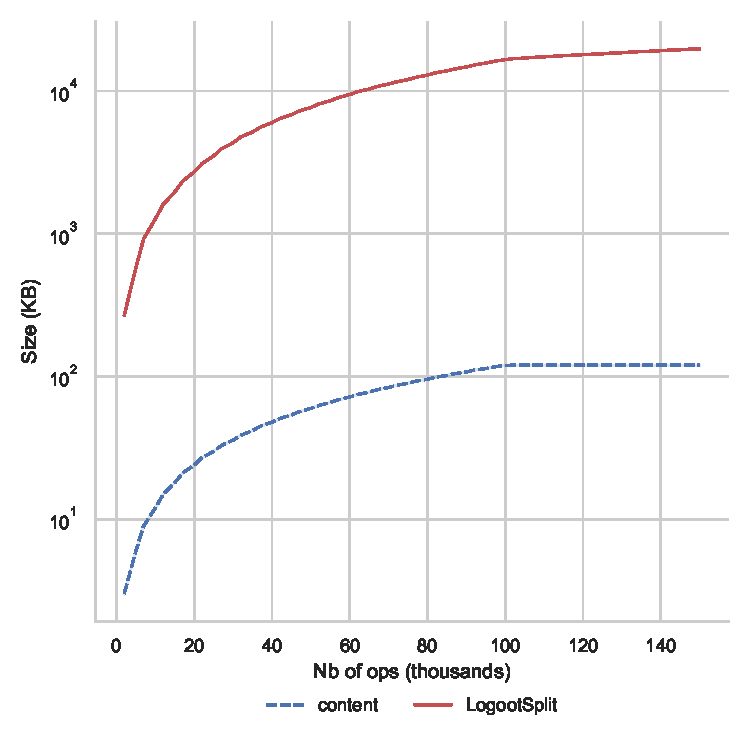
\includegraphics[trim=0cm 0.5cm 0cm 0cm, clip]{img/ls-vs-content-snapshot-sizes-7k5.pdf}
                }
                \caption{Taille du contenu comparée à la taille de la séquence LogootSplit}
            \end{figure}
        \end{column}
        \begin{column}{0.4\textwidth}
            \vspace{-2em}
            \begin{center}
                Diminution des performances du point de vue \alert{mémoire, calculs et bande-passante}
            \end{center}
        \end{column}
    \end{columns}
\end{frame}

\begin{frame}[fragile]{Comment réduire le surcoût ?}
    \metroset{block=transparent}
    \begin{block}{Solution naïve}
        \begin{figure}
            \resizebox{\textwidth}{!}{
              \begin{tikzpicture}
                \newcommand\nodeo[1]{
                    node[letter, label=#1:{$\trm{id}_1$}] {O}
                }
                \newcommand\noden[1]{
                    node[letter, label=#1:{$\trm{id}_2$}] {N}
                }
                \newcommand\nodee[1]{
                    node[letter, label=#1:{$\trm{id}_3$}] {E}
                }
                \newcommand\nodeebis[1]{
                    node[letter, label=#1:{$\trm{id}_{97}$}] {E}
                }
                \newcommand\nodenbis[1]{
                    node[letter, label=#1:{$\trm{id}_{98}$}] {N}
                }
                \newcommand\noded[1]{
                    node[letter, label=#1:{$\trm{id}_{99}$}] {D}
                }


                \newcommand\renoneend[1]{
                    node[block, label=#1:{$\trm{id}'_{begin..end}$}] {ONE$\cdots$END}
                }

                \newcommand\initialstate[3]{
                    \path
                    #1
                    ++#2
                    ++(0:0.5)
                    ++(#3:0.5) \nodeo{-#3}
                    ++(0:\widthletter) \noden{-#3}
                    ++(0:\widthletter) \nodee{-#3}
                    +(0:1.5 * \widthletter) node {$\cdots$}
                    ++(0:2 * \widthletter) \nodeebis{-#3}
                    ++(0:\widthletter) \nodenbis{-#3}
                    ++(0:\widthletter) \noded{-#3};
                }

                \newcommand\finalstate[3]{
                  \path
                  #1
                  ++#2
                  ++(0:0.5)
                  ++(#3:0.5) \renoneend{-#3};
                }

                \newcommand\offseta{ (90:0.7) }

                \path
                    node {\textbf{A}}
                    ++(0:0.5) node (a) {}
                    +(0:11) node (a-end) {}
                    +(0:1) node[point] (a-initial) {}
                    +(0:8) node (a-ren) {}
                    +(0:10) node (a-final) {};

                \initialstate{(a-initial)}{\offseta}{90};

                \draw[dotted] (a) -- (a-initial) (a-final) -- (a-end);

                \only<1,2>{
                    \draw[->, thick] (a-initial) -- (a-final);
                }
                \onslide<2->{
                    \finalstate{(a-ren)}{\offseta}{90};
                }
                \onslide<3->{
                    \path (a-ren) node[point, label=-170:{$?$}] {};
                    \draw[->, thick] (a-initial) --  (a-ren) -- (a-final);
                }
              \end{tikzpicture}
            }
          \end{figure}
          \begin{itemize}
            \item \alert{Convertir l'état} actuel\dots
            \item<2-> \dots \alert{en un état optimisé} (identifiants de taille minimale, moins de blocs)\dots
            \item<3-> \dots à l'aide d'une \alert{nouvelle opération}
          \end{itemize}
    \end{block}
\end{frame}

\subsection{RenamableLogootSplit}

\begin{frame}{Contribution : RenamableLogootSplit}
    \begin{itemize}
        \item CRDT pour le type Séquence qui incorpore un mécanisme de renommage
        \item Prend la forme d'une nouvelle opération : \ren
    \end{itemize}
    \begin{block}{Propriétés de l'opération \ren}
        \begin{itemize}
            \item Est déterministe
            \item Préserve l'intention des utilisateur-rices
            \item Préserve les propriétés de la séquence, \ie l'unicité et l'ordre de ses identifiants
            \item Commute avec les opérations \ins, \rmv mais aussi \ren concurrentes
        \end{itemize}
    \end{block}
\end{frame}

\subsection{Opération \emph{rename}}

\begin{frame}[fragile]{Opération \ren}
  \begin{figure}
    \resizebox{\textwidth}{!}{
      \begin{tikzpicture}
        \newcommand\nodeh[1]{
            node[letter, label=#1:{$\id{i}{B1}{0}$}] {H}
        }
        \newcommand\nodee[1]{
            node[letter, fill=\colorblockone, label=#1:{$\coloridone\id{i}{B1}{0}\id{f}{A1}{0}$}] {E}
        }
        \newcommand\nodelo[1]{
            node[block, label=#1:{$\id{i}{B1}{1..2}$}] {LO}
        }
        \newcommand\renh[1]{
            node[letter, fill=\colorblocktwo, label=#1:{$\coloridtwo\id{i}{A2}{0}$}] {H}
        }
        \newcommand\rene[1]{
            node[letter, fill=\colorblocktwo, label=#1:{$\coloridtwo\id{i}{A2}{1}$}] {E}
        }
        \newcommand\renl[1]{
            node[letter, fill=\colorblocktwo, label=#1:{$\coloridtwo\id{i}{A2}{2}$}] {L}
        }
        \newcommand\reno[1]{
            node[letter, fill=\colorblocktwo, label=#1:{$\coloridtwo\id{i}{A2}{3}$}] {O}
        }
        \newcommand\renhelo[1]{
            node[block, fill=\colorblocktwo, label=#1:{$\coloridtwo\id{i}{A2}{0..3}$}] {HELO}
        }

        \newcommand\initialstate[3]{
            \path
            #1
            ++#2
            ++(0:0.5)
            ++(#3:0.5) \nodeh{-#3}
            ++(0:\widthletter) \nodee{#3}
            ++(0:\widthletter) \nodelo{-#3};
        }

        \newcommand\stateh[3]{
            \path
            #1
            ++#2
            ++(0:0.5)
            ++(#3:0.5) \renh{-#3};
        }

        \newcommand\statehe[3]{
          \path
          #1
          ++#2
          ++(0:0.5)
          ++(#3:0.5) \renh{-#3}
          ++(0:\widthletter) \rene{-#3};
        }

        \newcommand\statehel[3]{
          \path
          #1
          ++#2
          ++(0:0.5)
          ++(#3:0.5) \renh{-#3}
          ++(0:\widthletter) \rene{-#3}
          ++(0:\widthletter) \renl{-#3};
        }

        \newcommand\statehelo[3]{
          \path
          #1
          ++#2
          ++(0:0.5)
          ++(#3:0.5) \renh{-#3}
          ++(0:\widthletter) \rene{-#3}
          ++(0:\widthletter) \renl{-#3}
          ++(0:\widthletter) \reno{-#3};
        }

        \newcommand\finalstate[3]{
          \path
          #1
          ++#2
          ++(0:0.5)
          ++(#3:0.5) \renhelo{-#3};
        }

        \newcommand\offseta{ (90:0.7) }

        \path
            node {\textbf{A}}
            ++(0:0.5) node (a) {}
            +(0:11) node (a-end) {}
            +(0:1) node[point] (a-initial) {}
            +(0:6) node[point] (a-ren-a1) {}
            +(0:10) node (a-final) {};

        \initialstate{(a-initial)}{\offseta}{90};

        \onslide<1-8>{\path (a-ren-a1) node[label=-170:{$\trm{ren}()$}, label={[xshift=0pt]-10:{$\trm{ren}(A,2)$}}] {};}

        \only<4>{\stateh{(a-ren-a1)}{\offseta}{90}};
        \only<5>{\statehe{(a-ren-a1)}{\offseta}{90};}
        \only<6>{\statehel{(a-ren-a1)}{\offseta}{90};}
        \only<7>{\statehelo{(a-ren-a1)}{\offseta}{90};}
        \onslide<8->{\finalstate{(a-ren-a1)}{\offseta}{90};}
        \only<9>{\path (a-ren-a1) node[label=-170:{$\trm{ren}()$}, label={[xshift=0pt]-10:{$\trm{ren}(A,2,\trm{renIds})$}}] {};}

        \draw[dotted] (a) -- (a-initial) (a-final) -- (a-end);
        \draw[->, thick] (a-initial) --  (a-ren-a1) -- (a-final);
      \end{tikzpicture}
    }
  \end{figure}
  \begin{itemize}
    \item<2-> Génère nouvel identifiant pour le 1er élément : \onslide<3->{$\id{i}{B1}{0} \to \id{i}{A2}{0}$}
    \item<4-> Puis génère identifiants contigus pour éléments suivants : \onslide<5->{$\id{i}{A2}{1}$}\onslide<6->{, $\id{i}{A2}{2}$}\onslide<7->{, \dots}
  \end{itemize}

  \onslide<8->{
    \begin{center}
      \alert{Regroupe tous les éléments en 1 unique bloc}
    \end{center}
  }

  \onslide<9->{
    \begin{block}{Pour plus tard :}
      \begin{itemize}
        \item Stocke identifiants ($[\id{i}{B1}{0},\id{i}{B1}{0}\id{f}{A1}{0},\dots]$) de l'état d'origine : $\trm{renIds}$
      \end{itemize}
  \end{block}
  }
\end{frame}

\subsection{Intégration des opérations \ins et \rmv concurrentes}

\begin{frame}[fragile]{Interactions avec opérations \ins et \rmv concurrentes}
  \begin{figure}
    \resizebox{\textwidth}{!}{
      \begin{tikzpicture}
        \newcommand\nodeh[1]{
            node[letter, label=#1:{$\id{i}{B1}{0}$}] {H}
        }
        \newcommand\nodee[1]{
            node[letter, fill=\colorblockone, label=#1:{$\coloridone\id{i}{B1}{0}\id{f}{A1}{0}$}] {E}
        }
        \newcommand\nodelo[1]{
            node[block, label=#1:{$\id{i}{B1}{1..2}$}] {LO}
        }
        \newcommand\renhelo[1]{
            node[block, fill=\colorblocktwo, label=#1:{$\coloridtwo\id{i}{A2}{0..3}$}] {HELO}
        }
        \newcommand\nodel[1]{
            node[letter, fill=\colorblockthree, label=#1:{$\coloridthree\id{i}{B1}{0}\id{m}{B2}{0}$}] {L}
        }
        \newcommand\crossl[1]{
            node[letter, cross, fill=\colorblockthree, label=#1:{$\coloridthree\id{i}{B1}{0}\id{m}{B2}{0}$}] {L}
        }

        \newcommand\initialstate[3]{
            \path
                #1
                ++#2
                ++(0:0.5)
                ++(#3:0.5) \nodeh{-#3}
                ++(0:\widthletter) \nodee{#3}
                ++(0:\widthletter) \nodelo{-#3};
        }

        \newcommand\statehelo[3]{
            \path
                #1
                ++#2
                ++(0:0.5)
                ++(#3:0.5) \renhelo{-#3};
        }

        \newcommand\insl[3]{
            \path
            #1
            ++#2
            ++(0:0.5)
            ++(#3:0.5) \nodeh{-#3}
            ++(0:\widthletter) \nodee{#3}
            ++(0:\widthletter) \nodel{-#3}
            ++(0:\widthletter) \nodelo{#3};
        }

        \newcommand\finalstate[3]{
            \path
                #1
                ++#2
                ++(0:0.5)
                ++(#3:0.5) \renhelo{-#3}
                ++(0:\widthblock) \nodel{#3};
        }

        \newcommand\finalstatecrossed[3]{
            \path
                #1
                ++#2
                ++(0:0.5)
                ++(#3:0.5) \renhelo{-#3}
                ++(0:\widthblock) \crossl{#3};
        }

        \newcommand\offseta{ (90:0.7) }
        \newcommand\offsetb{ (-90:0.7) }

        \path
            node {\textbf{A}}
            ++(0:0.5) node (a) {}
            +(0:16) node (a-end) {}
            +(0:1) node[point] (a-initial) {}
            +(0:6) node[point, label=-170:{$\trm{ren}()$}, label={[xshift=0pt]-10:{$\trm{ren}(A,2,\trm{renIds})$}}] (a-ren-a1) {}
            +(0:12) node (a-recv-ins-l) {}
            +(0:15) node (a-final) {};
        \path<3->
            (a-recv-ins-l) node[point] {};

        \initialstate{(a-initial)}{\offseta}{90};
        \statehelo{(a-ren-a1)}{\offseta}{90};
        \only<4>{\finalstate{(a-recv-ins-l)}{\offseta}{90};}
        \onslide<5->{\finalstatecrossed{(a-recv-ins-l)}{\offseta}{90};}

        \draw[dotted] (a) -- (a-initial) (a-final) -- (a-end);
        \draw<-2>[->, thick] (a-initial) --  (a-ren-a1) -- (a-final);
        \draw<3->[->, thick] (a-initial) --  (a-ren-a1) -- (a-recv-ins-l) -- (a-final);

        \path
            ++(270:2) node {\textbf{B}}
            ++(0:0.5) node (b) {}
            +(0:16) node (b-end) {}
            +(0:1) node[point] (b-initial) {}
            +(0:6) node (b-ins-l) {}
            +(0:15) node (b-final) {};
        \path<2->
            (b-ins-l) node[point, label=170:{$\trm{ins}(E \prec L \prec L)$}] {};
        \path<3->
            (b-ins-l) node[label={[xshift=45pt]10:{$\trm{ins}({\coloridthree\id{i}{B1}{0}\id{m}{B2}{0}},L)$}}] {};

        \initialstate{(b-initial)}{\offsetb}{-90};
        \onslide<2->{\insl{(b-ins-l)}{\offsetb}{-90};}

        \draw[dotted] (b) -- (b-initial) (b-final) -- (b-end);
        \draw<1>[->, thick] (b-initial) -- (b-final);
        \draw<2->[->, thick] (b-initial) --  (b-ins-l) -- (b-final);

        \draw<3->[->, dashed, shorten >= 1] (b-ins-l) -- (a-recv-ins-l);
      \end{tikzpicture}
    }
  \end{figure}
  \begin{itemize}
    \item Noeuds peuvent générer opérations concurrentes aux opérations \ren
    \item<5-> Opérations produisent anomalies si intégrées naïvement
  \end{itemize}
  \onslide<6>{
    \begin{center}
      \alert{Nécessité d'un mécanisme dédié}
    \end{center}
  }
\end{frame}

\begin{frame}{Mécanisme de résolution de conflits entre une opération \ren et une opération \ins ou \rmv}
    \begin{block}{Besoins}
        \begin{enumerate}
            \item
                \only<1>{Détecter les opérations concurrentes aux opérations \ren}
                \only<2>{\alert{Détecter les opérations concurrentes aux opérations \ren}}
            \item Prendre en compte effet des opérations \ren lors de l'intégration des opérations concurrentes
        \end{enumerate}
    \end{block}
\end{frame}

\begin{frame}[fragile]{Détection des opérations concurrentes à opération \ren}
    % \begin{center}
    %     \alert{Besoin de détecter opérations concurrentes à opération \ren}
    % \end{center}
    \vspace{-1.5em}
    \begin{figure}
        \resizebox{\textwidth}{!}{
          \begin{tikzpicture}
            \newcommand\nodeh[1]{
                node[letter, label=#1:{$\id{i}{B1}{0}$}] {H}
            }
            \newcommand\nodee[1]{
                node[letter, fill=\colorblockone, label=#1:{\coloridone$\id{i}{B1}{0}\id{f}{A1}{0}$}] {E}
            }
            \newcommand\nodelo[1]{
                node[block, label=#1:{$\id{i}{B1}{1..2}$}] {LO}
            }
            \newcommand\renhelo[1]{
                node[block, fill=\colorblocktwo, label=#1:{\coloridtwo$\id{i}{A2}{0..3}$}] {HELO}
            }
            \newcommand\nodel[1]{
                node[letter, fill=\colorblockthree,label=#1:{\coloridthree$\id{i}{B1}{0}\id{m}{B2}{0}$}] {L}
            }
            \newcommand\renhe[1]{
                node[block, fill=\colorblocktwo, label=#1:{\coloridtwo$\id{i}{A2}{0..1}$}] {HE}
            }
            \newcommand\renl[1]{
                node[letter, fill=\colorblockfour, label=#1:{\coloridfour$\id{i}{A2}{1}\id{i}{B1}{0}\id{m}{B2}{0}$}] {L}
            }
            \newcommand\renlo[1]{
                node[block, fill=\colorblocktwo, label=#1:{\coloridtwo$\id{i}{A2}{2..3}$}] {LO}
            }

            \newcommand\initialstate[3]{
                \path
                    #1
                    ++#2
                    ++(0:0.5)
                    ++(#3:0.5)
                    ++(0:1.25 * \widthoriginepoch) \nodeh{-#3}
                    ++(0:\widthletter) \nodee{#3}
                    ++(0:\widthletter) \nodelo{-#3};
            }

            \newcommand\initialstatewithepoch[3]{
                \path
                    #1
                    ++#2
                    ++(0:0.5)
                    ++(#3:0.5) node[epoch] {$\epoch{0}$}
                    ++(0:1.25 * \widthoriginepoch) \nodeh{-#3}
                    ++(0:\widthletter) \nodee{#3}
                    ++(0:\widthletter) \nodelo{-#3};
            }

            \newcommand\statehelo[3]{
                \path
                    #1
                    ++#2
                    ++(0:0.5)
                    ++(#3:0.5)
                    ++(0:1.18 * \widthepoch) \renhelo{-#3};
            }

            \newcommand\statehelowithepoch[3]{
                \path
                    #1
                    ++#2
                    ++(0:0.5)
                    ++(#3:0.5) node[epoch] {$\epoch{A2}$}
                    ++(0:1.18 * \widthepoch) \renhelo{-#3};
            }

            \newcommand\insl[3]{
                \path
                #1
                ++#2
                ++(0:0.5)
                ++(#3:0.5)
                ++(0:1.25 * \widthoriginepoch) \nodeh{-#3}
                ++(0:\widthletter) \nodee{#3}
                ++(0:\widthletter) \nodel{-#3}
                ++(0:\widthletter) \nodelo{#3};
            }

            \newcommand\inslwithepoch[3]{
                \path
                #1
                ++#2
                ++(0:0.5)
                ++(#3:0.5) node[epoch] {$\epoch{0}$}
                ++(0:1.25 * \widthoriginepoch) \nodeh{-#3}
                ++(0:\widthletter) \nodee{#3}
                ++(0:\widthletter) \nodel{-#3}
                ++(0:\widthletter) \nodelo{#3};
            }

            \newcommand\offseta{ (90:0.7) }
            \newcommand\offsetb{ (-90:0.7) }

            \path
                node {\textbf{A}}
                ++(0:0.5) node (a) {}
                +(0:15) node (a-end) {}
                +(0:1) node[point] (a-initial) {}
                +(0:7) node[point, label=-170:{$\trm{ren}()$}, ] (a-ren-a1) {}
                +(0:13) node[point] (a-recv-ins-l) {}
                +(0:14) node (a-final) {};
            \path<5>
                (a-ren-a1) node[label={[xshift=0pt]-10:{$\trm{ren}(\epoch{0}, A,2,\renids{A2})$}}] {};

            \onslide<1-2>{\initialstate{(a-initial)}{\offseta}{90};}
            \onslide<1-3>{\statehelo{(a-ren-a1)}{\offseta}{90};}
            \onslide<3->{\initialstatewithepoch{(a-initial)}{\offseta}{90};}
            \onslide<4->{\statehelowithepoch{(a-ren-a1)}{\offseta}{90};}

            \draw[dotted] (a) -- (a-initial) (a-final) -- (a-end);
            \draw[->, thick] (a-initial) --  (a-ren-a1) -- (a-recv-ins-l) -- (a-final);

            \path
                ++(270:2) node {\textbf{B}}
                ++(0:0.5) node (b) {}
                +(0:15) node (b-end) {}
                +(0:1) node[point] (b-initial) {}
                +(0:7) node[point, label=170:{$\trm{ins}(E \prec L \prec L)$}] (b-ins-l) {}
                +(0:14) node (b-final) {};
            \path<5>
                (b-ins-l) node[label={[xshift=45pt]10:{$\trm{ins}(\epoch{0}, {\coloridthree\id{i}{B1}{0}\id{m}{B2}{0}},L)$}}] {};


            \onslide<1-2>{
                \initialstate{(b-initial)}{\offsetb}{-90};
                \insl{(b-ins-l)}{\offsetb}{-90};
            }
            \onslide<3->{
                \initialstatewithepoch{(b-initial)}{\offsetb}{-90};
                \inslwithepoch{(b-ins-l)}{\offsetb}{-90};
            }

            \draw[dotted] (b) -- (b-initial) (b-final) -- (b-end);
            \draw[->, thick] (b-initial) --  (b-ins-l) -- (b-final);

            \draw[->, dashed, shorten >= 1] (b-ins-l) -- (a-recv-ins-l);
          \end{tikzpicture}
        }
    \end{figure}
    \metroset{block=transparent}
    \begin{block}<2->{Ajout mécanisme d'époques}
        \begin{itemize}
            \item<3-> Séquence commence à époque d'origine, notée $\epoch{0}$
            \item<4-> \ren font progresser à nouvelle époque, $\epoch{\trm{nodeId}~\trm{nodeSeq}}$
            \item<5-> Opérations labellisées avec époque de génération
        \end{itemize}
    \end{block}
\end{frame}

\begin{frame}{Mécanisme de résolution de conflits}
    \begin{block}{Besoins}
        \begin{enumerate}
            \item {\color{gray}Détecter les opérations concurrentes aux opérations \ren}
            \item \alert{Prendre en compte effet des opérations \ren lors de l'intégration des opérations concurrentes}
        \end{enumerate}
    \end{block}
\end{frame}

\begin{frame}[fragile]{Intégration des opérations \ins et \rmv concurrentes}
  \vspace{-1.5em}
  \begin{figure}
    \resizebox{\textwidth}{!}{
      \begin{tikzpicture}
        \newcommand\nodeh[1]{
            node[letter, label=#1:{$\id{i}{B1}{0}$}] {H}
        }
        \newcommand\nodee[1]{
            node[letter, fill=\colorblockone, label=#1:{\coloridone$\id{i}{B1}{0}\id{f}{A1}{0}$}] {E}
        }
        \newcommand\nodelo[1]{
            node[block, label=#1:{$\id{i}{B1}{1..2}$}] {LO}
        }
        \newcommand\renhelo[1]{
            node[block, fill=\colorblocktwo, label=#1:{\coloridtwo$\id{i}{A2}{0..3}$}] {HELO}
        }
        \newcommand\nodel[1]{
            node[letter, fill=\colorblockthree,label=#1:{\coloridthree$\id{i}{B1}{0}\id{m}{B2}{0}$}] {L}
        }
        \newcommand\renhe[1]{
            node[block, fill=\colorblocktwo, label=#1:{\coloridtwo$\id{i}{A2}{0..1}$}] {HE}
        }
        \newcommand\renl[1]{
            node[letter, fill=\colorblockfour, label=#1:{\coloridfour$\id{i}{A2}{1}\id{i}{B1}{0}\id{m}{B2}{0}$}] {L}
        }
        \newcommand\renlo[1]{
            node[block, fill=\colorblocktwo, label=#1:{\coloridtwo$\id{i}{A2}{2..3}$}] {LO}
        }

        \newcommand\statehelo[3]{
            \path
                #1
                ++#2
                ++(0:0.5)
                ++(#3:0.5) node[epoch] {$\epoch{A2}$}
                ++(0:1.18 * \widthepoch) \renhelo{-#3};
        }

        \newcommand\insl[3]{
            \path
            #1
            ++#2
            ++(0:0.5)
            ++(#3:0.5) node[epoch] {$\epoch{0}$}
            ++(0:1.25 * \widthoriginepoch) \nodeh{-#3}
            ++(0:\widthletter) \nodee{#3}
            ++(0:\widthletter) \nodel{-#3}
            ++(0:\widthletter) \nodelo{#3};
        }

        \newcommand\statehellowithoutid[3]{
            \path
            #1
            ++#2
            ++(0:0.5)
            ++(#3:0.5) node[epoch] {$\epoch{A2}$}
            ++(0:1.18 * \widthepoch) \renhe{-#3}
            ++(0:\widthblock) node[letter, fill=\colorblockfour, label=#3:{\coloridfour ?}] {L}
            ++(0:\widthletter) \renlo{-#3};
        }

        \newcommand\finalstate[3]{
            \path
                #1
                ++#2
                ++(0:0.5)
                ++(#3:0.5) node[epoch] {$\epoch{A2}$}
                ++(0:1.18 * \widthepoch) \renhe{-#3}
                ++(0:\widthblock) \renl{#3}
                ++(0:\widthletter) \renlo{-#3};
        }

        \newcommand\offseta{ (90:0.7) }
        \newcommand\offsetb{ (-90:0.7) }

        \path
            node {\textbf{A}}
            ++(0:0.5) node (a) {}
            +(0:13) node (a-end) {}
            +(0:1) node[point] (a-initial) {}
            +(0:7) node[point] (a-recv-ins-l) {}
            +(0:12) node (a-final) {};

        \statehelo{(a-initial)}{\offseta}{90};
        \statehellowithoutid{(a-recv-ins-l)}{\offseta}{90};
        %\finalstate{(a-recv-ins-l)}{\offseta}{90};

        \draw[dotted] (a) -- (a-initial) (a-final) -- (a-end);
        \draw[->, thick] (a-initial) -- (a-recv-ins-l) -- (a-final);

        \path
            ++(270:2) node {\textbf{B}}
            ++(0:0.5) node (b) {}
            +(0:13) node (b-end) {}
            +(0:1) node[point, label={[xshift=45pt]10:{$\trm{ins}(\epoch{0}, {\coloridthree\id{i}{B1}{0}\id{m}{B2}{0}},L)$}}] (b-initial) {}
            +(0:12) node (b-final) {};

        \insl{(b-initial)}{\offsetb}{-90};

        \draw[dotted] (b) -- (b-initial) (b-final) -- (b-end);
        \draw[->, thick] (b-initial) -- (b-final);

        \draw[->, dashed, shorten >= 1] (b-initial) -- (a-recv-ins-l);
      \end{tikzpicture}
    }
  \end{figure}
  \metroset{block=transparent}
  \begin{block}<2->{Ajout d'un mécanisme de transformation des opérations \ins et \rmv concurrentes}
    \begin{itemize}
        \item<3-> Prend la forme de l'algorithme \texttt{renameId}
        \item<4> \alert{Inclure l'effet de l'opération \ren dans l'opération transformée}
    \end{itemize}
  \end{block}
\end{frame}

\begin{frame}[fragile]{Exemple de \texttt{renameId}}
    \vspace{-0.5 em}
    \begin{figure}
      \resizebox{0.9 \textwidth}{!}{
        \begin{tikzpicture}
          \newcommand\nodeh[1]{
              node[letter, label=#1:{$\id{i}{B1}{0}$}] {H}
          }
          \newcommand\nodee[1]{
              node[letter, fill=\colorblockone, label=#1:{\coloridone$\id{i}{B1}{0}\id{f}{A1}{0}$}] {E}
          }
          \newcommand\nodelo[1]{
              node[block, label=#1:{$\id{i}{B1}{1..2}$}] {LO}
          }
          \newcommand\renhelo[1]{
              node[block, fill=\colorblocktwo, label=#1:{\coloridtwo$\id{i}{A2}{0..3}$}] {HELO}
          }
          \newcommand\nodel[1]{
              node[letter, fill=\colorblockthree,label=#1:{\coloridthree$\id{i}{B1}{0}\id{m}{B2}{0}$}] {L}
          }
          \newcommand\renhe[1]{
              node[block, fill=\colorblocktwo, label=#1:{\coloridtwo$\id{i}{A2}{0..1}$}] {HE}
          }
          \newcommand\renl[1]{
              node[letter, fill=\colorblockfour, label=#1:{\coloridfour$\id{i}{A2}{1}\id{i}{B1}{0}\id{m}{B2}{0}$}] {L}
          }
          \newcommand\renlo[1]{
              node[block, fill=\colorblocktwo, label=#1:{\coloridtwo$\id{i}{A2}{2..3}$}] {LO}
          }

          \newcommand\statehelo[3]{
              \path
                  #1
                  ++#2
                  ++(0:0.5)
                  ++(#3:0.5) node[epoch] {$\epoch{A2}$}
                  ++(0:1.18 * \widthepoch) \renhelo{-#3};
          }

          \newcommand\insl[3]{
              \path
              #1
              ++#2
              ++(0:0.5)
              ++(#3:0.5) node[epoch] {$\epoch{0}$}
              ++(0:1.25 * \widthoriginepoch) \nodeh{-#3}
              ++(0:\widthletter) \nodee{#3}
              ++(0:\widthletter) \nodel{-#3}
              ++(0:\widthletter) \nodelo{#3};
          }

          \newcommand\statehellowithoutid[3]{
              \path
              #1
              ++#2
              ++(0:0.5)
              ++(#3:0.5) node[epoch] {$\epoch{A2}$}
              ++(0:1.18 * \widthepoch) \renhe{-#3}
              ++(0:\widthblock) node[letter, fill=\colorblockfour, label=#3:{\coloridfour ?}] {L}
              ++(0:\widthletter) \renlo{-#3};
          }

          \newcommand\finalstate[3]{
              \path
                  #1
                  ++#2
                  ++(0:0.5)
                  ++(#3:0.5) node[epoch] {$\epoch{A2}$}
                  ++(0:1.18 * \widthepoch) \renhe{-#3}
                  ++(0:\widthblock) \renl{#3}
                  ++(0:\widthletter) \renlo{-#3};
          }

          \newcommand\offseta{ (90:0.7) }
          \newcommand\offsetb{ (-90:0.7) }

          \path
              node {\textbf{A}}
              ++(0:0.5) node (a) {}
              +(0:13) node (a-end) {}
              +(0:1) node[point] (a-initial) {}
              +(0:7) node[point] (a-recv-ins-l) {}
              +(0:12) node (a-final) {};

          \statehelo{(a-initial)}{\offseta}{90};
          \onslide<1-4>{
            \statehellowithoutid{(a-recv-ins-l)}{\offseta}{90};
          }
          \onslide<5>{
            \finalstate{(a-recv-ins-l)}{\offseta}{90};
          }

          \draw[dotted] (a) -- (a-initial) (a-final) -- (a-end);
          \draw[->, thick] (a-initial) -- (a-recv-ins-l) -- (a-final);

          \path
              ++(270:2) node {\textbf{B}}
              ++(0:0.5) node (b) {}
              +(0:13) node (b-end) {}
              +(0:1) node[point, label={[xshift=45pt]10:{$\trm{ins}(\epoch{0}, {\coloridthree\id{i}{B1}{0}\id{m}{B2}{0}},L)$}}] (b-initial) {}
              +(0:12) node (b-final) {};

          \insl{(b-initial)}{\offsetb}{-90};

          \draw[dotted] (b) -- (b-initial) (b-final) -- (b-end);
          \draw[->, thick] (b-initial) -- (b-final);

          \draw[->, dashed, shorten >= 1] (b-initial) -- (a-recv-ins-l);
        \end{tikzpicture}
      }
    \end{figure}
    \vspace{-1em}
    \textbf{Rappel : }
    \begin{equation*}
        \renids{A2} = [\id{i}{B1}{0},\only<2>{{\coloridone\id{\mathbf{i}}{\mathbf{B1}}{\mathbf{0}}\id{\mathbf{f}}{\mathbf{A1}}{\mathbf{0}}}}\only<3,4,5>{{\coloridone\id{i}{B1}{0}\id{f}{A1}{0}}}\only<1>{\id{i}{B1}{0}\id{f}{A1}{0}},\id{i}{B1}{1},\id{i}{B1}{2}]
    \end{equation*}
    \vspace{-1em}
    \begin{block}{Exemple avec {$\coloridone\id{i}{B1}{0}\id{m}{B2}{0}$}}
      \begin{itemize}
        \item<2-> Rechercher son prédecesseur dans $\renids{A2}$ : $\coloridone\id{i}{B1}{0}\id{f}{A1}{0}$
        \item<3-> Utiliser son index ($\coloridtwo 1$) pour calculer équivalent à époque $\epoch{A2}$ : $\coloridtwo\id{i}{A2}{1}$
        \item<4-> Préfixer {$\coloridthree\id{i}{B1}{0}\id{m}{B2}{0}$} par ce dernier : $\coloridfour\id{i}{A2}{1}$$\coloridthree\id{i}{B1}{0}\id{m}{B2}{0}$
      \end{itemize}
    \end{block}
  \end{frame}
